This chapter aims to review some of the fundamental methodological choices of the framework. For more details you can refer to the bibliography.

\section{Multiple Forwarding Curves and One Discounting Curve}

The Rate Curve Framework is (obviously) a Multi-Curve Framework. For each currency we typically have multiple Forwarding Curves, each one linked to a specific underlying index of given tenor. For example in the EUR market case we have five curves $C_{ON}$,$C_{1M}$,$C_{3M}$,$C_{6M}$,$C_{12M}$ with underlying indexes Eonia, Euribor 1M, Euribor 3M, Euribor 6M, Euribor 12M respectevely. Curves reference date is the start date of the spot calibrating instruments (forwarding has no meaning before this date).

Discount factors entering into the pricing formulas of calibrating instruments could be taken 
\begin{itemize}
\item from a predetermined discounting curve ({\it exogenous discounting}): discount factors are an input of the calibration process as well as market quotes;
\item from the forwarding curve itself ({\it endogenous discounting}): discount factors are an output of the calibration process.
\end{itemize}
Discounting curve reference date is today because we want present values referring to today.

All calibrating instruments are traded on regulated markets (Futures) or collateralized with daily margination at the overnight collateral rate  (FRA, Swaps and Basis Swaps). This is why the ON Curve usually plays the role of Discounting Curve (as well as the role of Forwarding Curve for its specific tenor). Once calibrated, all these curves are used to price and hedge collateralized products. The old Standard curve still plays the role of Discounting Curve for non-collateralized products and this is way inside our framework is defined also one Standard Curve for each currency. Even in this case all the Forwarding Curves are calibrated with exogenous OIS discounting (and not Standard Discounting). Finally we notice that
\begin{itemize}
\item the OIS curve and the corresponding forwarding curves are calibrated on Excel following the best practices (homogeneous instruments selection, synthetic deposits construction, choice of the best algorithm and interpolation method) and then contributed to the front office systems (through the process described in Chapter \ref{chap:1});  
\item Standard Curves are a mere replica of what has been configured inside the systems and are not used for contribution purposes.
\end{itemize}

We do not add other details but you can refer (for example) to \cite{ametranobianchetti} and \cite{henrard} for more details about foundations of multi-curve framework.

\section{Curves Description}\label{sec:description}

\subsection{Discounts, Zero Rates, Forward Rates}

In order to present the available descriptions for our curves we have to take a step back to the old one-curve world. The general idea of the one-curve framework is that all interest rate derivatives depend on only one curve described in terms of discount factors. If $t$ is our reference date, the discount factor $P(t;s)$ for a maturity $s\geq t$ is the price in $t$ of an instrument which pays 1 unit of currency in $s$. Starting from discount factors you can define simple zero rates, compounded zero rates (with frequency $m$) and continuously compounded zero rates via equations
\begin{align}
P(t;s)&=\frac{1}{1+z_{s}(t;s)\tau(t,s)}\label{eq:disc1}\\ 
P(t;s)&=\left(\frac{1}{1+z_{c}(t;s)/m}\right)^{m\tau(t,s)}\label{eq:disc2}\\ 
P(t;s)&=e^{-z(t;s)\tau(t,s)}\label{eq:disc3}
\end{align}
Simple rates and compounded rates are real objects: they are quoted by the market (directly or indirectly) and the corresponding day count convention $\tau$ is also defined by the market. Continuously compounded rates, instead, are only a mathematical abstraction (notice that they can be defined as the limit of compounded rates when $m \rightarrow \infty$); usually in this case $\tau$ is a specific strictly monotone day count convention (for example $Act/365$) in order to ensure that every date $s$ is mapped to a unique time $\tau(t,s)$.

We now define different types of forward rates. In order to do this, we have to fix two futures dates $s_{1},s_{2}$ with $t<s_{1}<s_{2}$ and a day count convention $\tau$. It is not possible to define forward rates without fixing a triplet $(s_{1},s_{2},\tau)$.

\subsubsection{Continuous Forward Rates}
A {\it continuous forward rate} $F_{c}(t;s_{1},s_{2})$ is defined as the future zero rate implied by today�s (unique) term structure of zero rates assuming continuous compounding. By no arbitrage
\begin{equation}\label{eq:contfwd}
e^{z(t;s_{1})\tau(t,s_{1})}e^{F_{c}(t;s_{1},s_{2})\tau(s_{1},s_{2})}=e^{z(t;s_{2})\tau(t,s_{2})}
\end{equation}
Equivalently
\begin{equation}\label{eq:contfwd1}
\begin{split}
F_{c}(t;s_{1},s_{2})&=\frac{z(t;s_{2})\tau(t,s_{2})-z(t;s_{1})\tau(t,s_{1})}{\tau(s_{1},s_{2})}\\
&\stackrel{\ref{eq:disc3}}{=}\frac{1}{\tau(s_{1},s_{2})}\ln \left(\frac{P(t;s_{1})}{P(t;s_{2})}\right)
\end{split}
\end{equation}
that defines $F_{c}$ in terms of discount factors and continuous compounded zero rates.

\subsubsection{Simple Forward Rates}
Similarly, a {\it simple forward rate} $F(t;s_{1},s_{2})$ is defined by
\begin{equation}\label{eq:simpfwd}
(1+z_{s}(t;s_{1})\tau(t,s_{1}))(1+F(t;s_{1},s_{2})\tau(s_{1},s_{2}))=1+z_{s}(t;s_{2})\tau(t,s_{2})
\end{equation}
Using equations \ref{eq:disc1} and \ref{eq:disc3} we have
\begin{equation}\label{eq:7bis}
F(t;s_{1},s_{2})=\frac{1}{\tau(s_{1},s_{2})}\left(\frac{P(t;s_{1})}{P(t;s_{2})}-1\right)=
\frac{1}{\tau(s_{1},s_{2})}\left(e^{z(t;s_{2})\tau(t,s_{2})-z(t;s_{1})\tau(t,s_{1})}-1\right)
\end{equation}
that defines $F$ in terms of discount factors and continuous compounded zero rates.

\subsubsection{Instantaneous Forward Rates}

An {\it instantaneous forward rate} is the continuous forward rate that applies for an infinitesimal period. It is defined by the following equation
\begin{equation}\label{eq:13}
f(t,s):=\lim_{s_{2}\rightarrow s_{1}} F_{c}(t;s_{1},s_{2})\stackrel{\ref{eq:contfwd1}}{=}\frac{d}{ds}\left(z(t;s)\tau(t,s)\right)
\end{equation}
By integrating
\begin{equation}\label{eq:basta}
\int_{t}^{s}f(t;u)du=z(t;s)\tau(t,s)
\end{equation}
and also
\begin{equation}\label{eq:bastabasta}
\int_{s_{1}}^{s_{2}}f(t;u)du=z(t;s_{2})\tau(t,s_{2})-z(t;s_{1})\tau(t,s_{1})
\end{equation}
From equations \ref{eq:contfwd1} and \ref{eq:bastabasta} we have
\begin{equation}\label{eq:12}
F_{c}(t;s_{1},s_{2})=\frac{1}{\tau(s_{1},s_{2})}\left(\int_{s_{1}}^{s_{2}}f(t;u)du\right)
\end{equation}
which shows that the average of the instantaneous forward rate over any interval $[s_{1},s_{2}]$ is equal to the continuous forward rate for that interval. From equations \ref{eq:7bis} and \ref{eq:bastabasta} we have 
\begin{equation}\label{eq:7}
F(t;s_{1},s_{2})=\frac{1}{\tau(s_{1},s_{2})}\left(e^{\int_{s_{1}}^{s_{2}}f(t;u)du}-1\right)
\end{equation}
which shows that simple forward rates are a continuous function of integrated instantaneous forward rates.

We have finally obtained the following important relationship between discount factors, continuously compounded zero rates and instantaneous forward rates
\begin{equation}\label{eq:5}
P(t;s)=e^{-z(t;s)\tau(t,s)}=e^{-\int_{t}^{s}f(t;u)du}
\end{equation}
or equivalently
\begin{equation}\label{eq:10}
-\ln P(t;s)=z(t;s)\tau(t,s)=\int_{t}^{s}f(t;u)du
\end{equation}
So we have at least three possible ways to describe our unique curve: through discount factors, through continuous compounded zero rates and through instantaneous forward rates. In formulas
\begin{align*}
C(t)&=\{s\rightarrow P(t;s)|s\geq t\}\\
C(t)&=\{s\rightarrow z(t;s)|s> t\}\\
C(t)&=\{s\rightarrow f(t;s)|s> t\}
\end{align*}
The three descriptions are almost equivalent; the only difference is that only discount factors are well defined when $s=t$ and we have $P(t;t)=1$.

We now come back to our multi-curve framework.

\subsection{Reasonable description through forward rates}

Each rate curve $C_{x}$ of the framework is a forwarding curve linked to a specific tenor $x$. The most natural description should be the one that models directly forward rates because the market quotes forward rates (and not other quantities like discount factors). Forward rates directly quoted by the market through FRA, Futures and indirectly through Interest Rates Swaps and Basis Swaps, are simple forward rates corresponding to a triplet $(s,s+x,\tau_{x})$ where $s\geq t$ and $\tau_{x}$ is the specific day count convention related to the underlying index of each instrument (example: Euribor $xM$). So our curve $C_{x}$ should be described by
\begin{equation}\label{eq:1}
C_{x}(t)=\{s\rightarrow F_{x}(t;s,s+x)|s\geq t\}
\end{equation}
Unfortunately, this is not the commonly used approach. 

\subsection{Classical description through pseudo-discount factors}

Equations \ref{eq:7bis}, \ref{eq:7} and \ref{eq:5} can be extended to multi-curve framework as follows: 
\begin{align}
F_{x}(t;s_{1},s_{2})&=\frac{1}{\tau(s_{1},s_{2})}\left(\frac{P_{x}(t;s_{1})}{P_{x}(t;s_{2})}-1\right)=\frac{1}{\tau(s_{1},s_{2})}\left(e^{\int_{s_{1}}^{s_{2}}f_{x}(t;u)du}-1\right) \label{eq:fwd}\\
P_{x}(t;s)&=e^{-z_{x}(t;s)\tau(t,s)}=e^{-\int_{t}^{s}f_{x}(t;u)du} \label{eq:8}
\end{align}
These are only definitions. The only real quantity, as said before, is the simple forward rate $F_{x}(t;s,s+x)$ quoted by the market which thus satisfies
\begin{equation}\label{eq:2}
\begin{split}
F_{x}(t;s,s+x)&=\frac{1}{\tau_{x}(s,s+x)}\left(\frac{P_{x}(t;s)}{P_{x}(t;s+x)}-1\right)\\
&=\frac{1}{\tau_{x}(s,s+x)}\left(e^{\int_{s}^{s+x}f_{x}(t;u)du}-1\right)
\end{split}
\end{equation}
Last equation is really similar to equation \ref{eq:7bis} but the substance of these new relation is totally different. More precisely
\begin{itemize}
\item single-curve equation is the result obtained from no arbitrage condition;
\item multi-curve equation is merely the definition of a {\it pseudo-discount factors} function $P_{x}(t;s)$.
\end{itemize}
To clarify this concept we can make the following example. In the old single-curve world, before 2007 crisis, in the EUR market we could calculate the forward rate $F(t;t+3M,t+6M)$ starting from the values $P(t;t+3M)$ and $P(t;t+6M)$ deduced from Euribor $3M$ and Euribor $6M$ fixings with a no arbitrage condition; the resulting value was in line with the market quote of the $3X6$ FRA. With the large Basis Swap spreads presently quoted on the market this relation is no more valid: if we calculate the $3X6$ FRA implicit in Euribor 6M and Euribor 3M fixings (as explained above) we do not obtain the $3X6$ FRA quoted by the market (see Figure \ref{fig:example}). We have to define two synthetic quantities $P_{3M}(t;t,t+3M)$ and $P_{3M}(t;t+6M)$ to make the old relationship still valid.
\begin{figure}
\centering
\begin{subfigure}[b]{\textwidth}
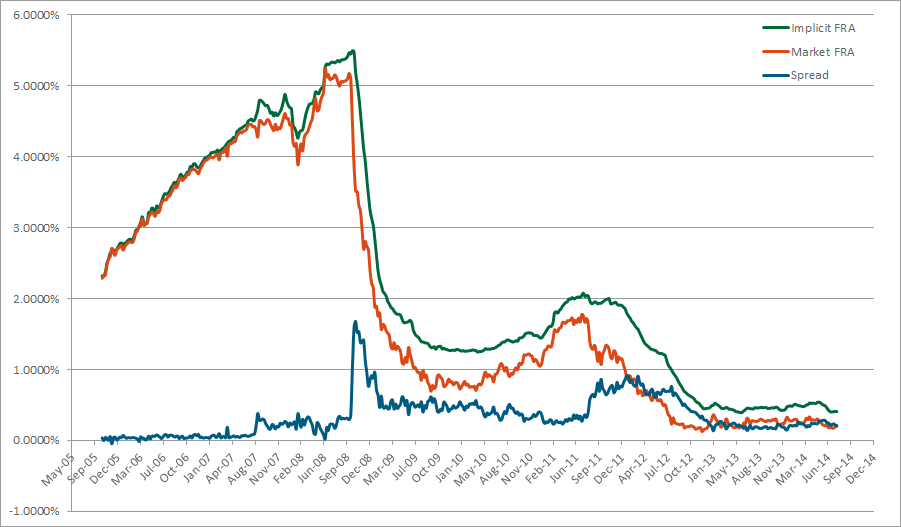
\includegraphics[width=\textwidth]{images/example1.png}
\end{subfigure}
\begin{subfigure}[b]{\textwidth}
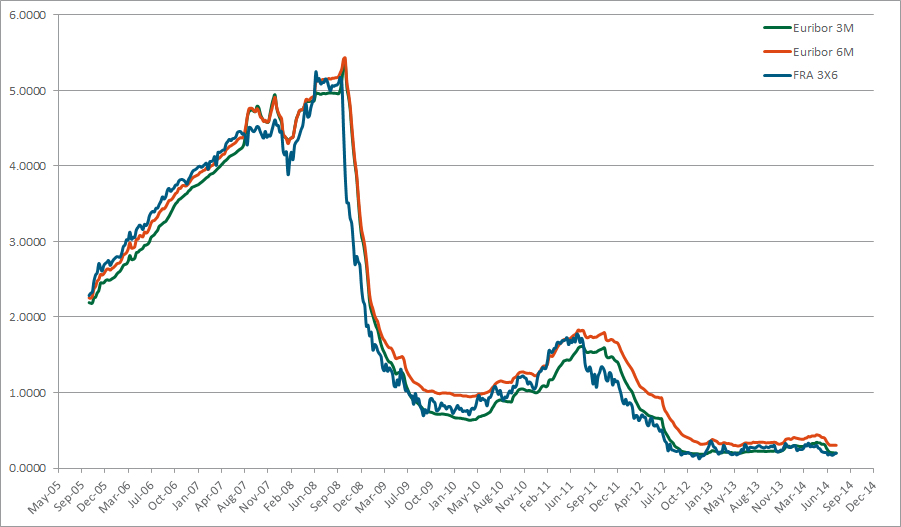
\includegraphics[width=\textwidth]{images/example2.png}
\end{subfigure}
\caption{After summer 2007 the $3X6$ FRA implicit in Euribor 6M and Euribor 3M fixings it was no longer consistent with the $3X6$ FRA quoted by the market. The large Basis Swap spread observed were an evidence of the need of multiple curves, one for each tenor. It was not a correlation break!}
\label{fig:example}
\end{figure}

Looking at equation \ref{eq:2} we notice that it is always possible to calculate a simple forward rates curve $\{s\rightarrow F_{x}(t;s,s+x)|s\geq t\}$ if a pseudo-discount factors curve $\{s\rightarrow P_{x}(t;s)|s\geq t\}$ is given but this is not our case. Conversely, it is not possible to deduce a unique pseudo-discount factors curve starting form a simple forward rates curve and this is due to the arbitrariness of the equation itself: a simple forward rate defines the ratio of two pseudo-discount factors and not a unique pseudo-discount factor. In this case, to define uniquely pseudo-discount factors we have to add other conditions, for example fixing their shape on the first $x$-interval $[t,Spot(today)+x)$ (remember that the reference date $t$ is today or the spot date referring to today). If we know the function $\{s\rightarrow P_{x}(t;s)|t\leq s\leq Spot(today)+x\}$ we can deduce the whole structure via equation \ref{eq:2}.

The discussion above has proved that for each forward curve $C_{x}$ we have the following alternative (almost equivalent) descriptions: 
\begin{align}\label{eq:9}
C_{x}(t)&=\{s\rightarrow P_{x}(t;s)|s\geq t\} \\
C_{x}(t)&=\{s\rightarrow z_{x}(t;s)|s> t\} \\
C_{x}(t)&=\{s\rightarrow f_{x}(t;s)|s> t\}
\end{align}
The advantage of one of this descriptions (compared to a direct forward rates description) is that it can be used to calibrate forward curves inside our legacy systems, that are linked to the old single-curve framework. On the other hand the drawbacks are obvious. First of all, you are not modelling directly the market quantities, the ones on which we have some intuition (the forward rates). Secondly, as said before, the function $P_{x}(t,s)$ has an arbitrary part of length $x$ that must be chosen. When $x=ON$ this arbitrary part is really small (few days) and it can be fixed with some market quotes. So in this case we can use the pseudo-discount factors description without problems at all; also this description is consistent with the role of $C_{ON}$ as discount curve of the framework (in this case pseudo-discount factors are real discount factors!). For the other tenors we will have to introduce synthetic deposits in order to manage this arbitrariness.
      
\section{Algorithms: Best Fit vs Exact Fit}\label{sec:algo}

There are two main classes of curves construction algorithms. The common feature is that both classes require a set of $N$ pre-selected market instruments.

A {\it best-fit algorithm} assumes a functional form for the curve $C_{x}$ and calibrates its parameters using the pre-selected instruments. It is very popular due to the smoothness of the curve, calibration easiness and intuitive financial interpretation of functional form parameters but it has a big drawback: usually there are more instruments than parameters so that the result of the calibration is not a perfect reprice of the whole set of instruments but a minimization of the repricing error. This is way the quality of a best-fit is not good enough for trading purposes in liquid markets, where a basis point quarter can make the difference.

{\it Exact-fit algorithms}, instead, fix the yield curve on a time grid of $N$ points (or {\it pillars}) in order to exactly reprice the selected instruments. An interpolation method is required to determine curve values between pillars. Usually the algorithm is incremental, building the curve step-by-step with the increasing maturity of the ordered instruments ({\it bootstrap} approach).

The interpolation method is intimately connected to the bootstrap and plays a fundamental role also during bootstrapping, not just after that. The calibration proceeds with incomplete information: in order to determine each pillar value, the already bootstrapped part of the curve has to be used, not only pillar values but also intermediate interpolated ones (see \cite{haganwest} for a practical example of this interaction between interpolation and bootstrap). 

Usually the set of bootstrapping instruments defines the time grid used for bootstrapping: each pillar is the maturity date or the last relevant date of the corresponding instrument. But this is not the only available choice: one can define a time grid of $N$ {\it custom dates} providing that each of these dates is earlier than the last relevant date of the corresponding instrument.  

Henceforward we restrict ourselves to the exact curve calibration problem.

\section{Interpolation}\label{sec:interpolation}

When we speak about interpolation we mean two distinct objects:
\begin{itemize}
\item the quantity to be interpolated;
\item the interpolation scheme.
\end{itemize}

The quantity to be interpolated is chosen according to curve's description. If we use a description through forward rates, the most reasonable quantity to be interpolated is the forward rate itself: in this way interpolation schemes and constraints can be imposed directly on market quantities. If we have to use a description through pseudo-discount factors (and this is our case) we have the following main choices: discount factors, zero rates, instantaneous forward rates. Another choice could be the logarithm of discount factor, that is the product between zero rate and time (see equation \ref{eq:8}).

Once the quantity to be interpolated is chosen, an interpolation scheme must be used to estimate curve values between pillars. There are two big classes of schemes:
\begin{itemize}
\item local schemes: each intermediate point depends only on its bracketing pillars;
\item global schemes: each intermediate point depends on points outside the interval defined by its neighborhoods pillars.
\end{itemize}
A typical example of local scheme is the linear one; cubic splines are examples of global interpolations. Notice that when bootstrapping with a local interpolation the curve's shape between two calibrated pillars can no longer change. If the interpolation method is global, the curve changes continuously until the end of the procedure because the shape of the part of the curve already bootstrapped is altered by the addition of further pillars. In this case, after a first bootstrap which might even use a local interpolation scheme, the resulting complete grid is altered one pillar at time until convergence is reached with a given precision. The first cycle can be even replaced by a good grid guess, for example the grid previous state. Also, with a global interpolation, the computational performance of bootstrapping algorithm is lowered, with the most important effects observed during sensitivities calculation.

The criteria used to analyse the interpolation techniques usually fall into one of the following two categories:
\begin{itemize}
\item the quality of the forward rates: in this case we are looking at the curve as an "accounting" tool and we are trying to answer the question "How good the forward rates look?"; 
\item the quality of the implied hedging strategies: in this case we are looking at the curve as a "risk management" tool and we are trying to answer the question "Are the implied hedging quantities reasonable and stable?"
\end{itemize}
Sometimes an interpolation method is good to build forward rates but not good from an hedging point of view. It is not impossible to use different interpolation schemes, one for each function, but this creates inconsistencies and is not advisable. The only way is to find a compromise.

We now describe some interpolation techniques (that is, quantity to be interpolated plus an interpolation scheme) trying to analyse the first aspect, that is the quality of discrete forward rates; hedging strategies will be discussed in a separate section. Since each simple forward rate is approximately the integral of instantaneous forward rates (remember equation \ref{eq:fwd}), we will analyze the smoothness of simple forward rates computing instantaneous forward rates via equation \ref{eq:13}. The starting point is a set of known curve's points $\left\{ (t_{i},y_{i}=y(t_{i}))\right\}_{i=1,...,N}$ where $y$ represent the quantity to be interpolated as defined above. $t_{0}$ will be the reference date.

\subsection{Linear Interpolation}

For $t \in [t_{i-1}, t_{i}]$ the interpolation formula is
$$
y(t)=\frac{t-t_{i-1}}{t_{i}-t_{i-1}}y(t_{i})+\frac{t_{i}-t}{t_{i}-t_{i-1}}y(t_{i-1})
$$
\subsubsection{On Zero Rates}

Let $y(t)=z(t_{0};t)\equiv z(t)$. Since $z(t)$ is piecewise linear also $f(t_{0},t)\equiv f(t)$ is piecewise linear because it is the derivative of the piecewise quadratic function $z(t)t$. In formulas
$$
z(t)t=\frac{t-t_{i-1}}{t_{i}-t_{i-1}}z(t_{i})t+\frac{t_{i}-t}{t_{i}-t_{i-1}}z(t_{i-1})t
$$
and
$$
f(t)=\frac{d}{dt}z(t)t=\frac{2t-t_{i-1}}{t_{i}-t_{i-1}}z(t_{i})+\frac{t_{i}-2t}{t_{i}-t_{i-1}}z(t_{i-1})
$$
But there is a difference. While $z(t)$ is $C^{0}$ on $[t_{0},t_{N}]$, this is not the case for $f(t)$ that presents a jump at each node; in fact values
$$
f(t_{i}^{+})=\lim_{t\rightarrow t_{i}}\left(\frac{2t-t_{i-1}}{t_{i}-t_{i-1}}z(t_{i})+\frac{t_{i}-2t}{t_{i}-t_{i-1}}z(t_{i-1})\right)=
\frac{2t_{i}-t_{i-1}}{t_{i}-t_{i-1}}z(t_{i})-\frac{t_{i}}{t_{i}-t_{i-1}}z(t_{i-1})
$$
and
$$
f(t_{i}^{-})=\lim_{t\rightarrow t_{i}}\left(\frac{2t-t_{i}}{t_{i+1}-t_{i}}z(t_{i+1})+\frac{t_{i+1}-2t}{t_{i+1}-t_{i}}z(t_{i})\right)=
-\frac{t_{i}}{t_{i+1}-t_{i}}z(t_{i+1})+\frac{t_{i+1}-2t_{i}}{t_{i+1}-t_{i}}z(t_{i})
$$
are different. Simple forward rates are obtained integrating $f(t)$ on a "rolling" interval of length $x$ (see equation \ref{eq:fwd}); thus they are smoother than instantaneous forward rates. In particular, $F_{x}(t;s,s+x)$ is $C^{0}$ with a "sawtooth" shape (see Figure \ref{fig:2}: we use daily forward rates as best proxy for instantaneous forward rates). This is clearly not the best interpolation method because the resulting forward rates have an improbable shape. 
\begin{figure}
\centering
\begin{subfigure}[b]{0.8\textwidth}
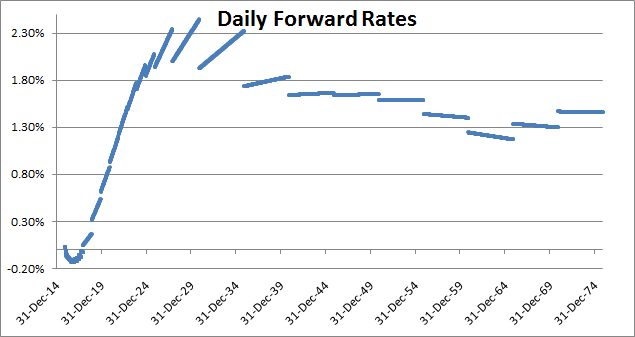
\includegraphics[width=\textwidth]{images/2a.png}
\caption{Piecewise Linear Daily Forward Rates}
\label{fig:2a}
\end{subfigure}
\begin{subfigure}[b]{0.8\textwidth}
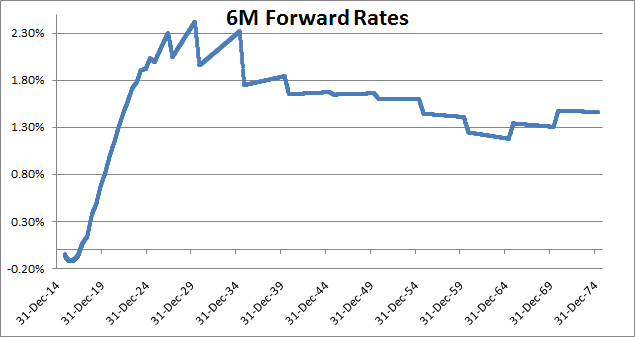
\includegraphics[width=\textwidth]{images/2b.png}
\caption{Sawtooth 6M Forward Rates}
\label{fig:2b}
\end{subfigure}
\caption{Euribor 6M Curve with Linear interpolation on Zero Rates}
\label{fig:2}
\end{figure}

\subsubsection{On Log of Discount Factors}

If $y(t)=\ln P(t_{0};t)\equiv \ln P(t)$ we have
$$
z(t)t=-\ln P(t)=-\frac{t-t_{i-1}}{t_{i}-t_{i-1}}\ln P(t_{i})-\frac{t_{i}-t}{t_{i}-t_{i-1}}\ln P(t_{i-1})
$$
Using equation \ref{eq:13} we get
$$
f(t)=\frac{d}{dt} z(t)t=\frac{-\ln P(t_{i})+\ln P(t_{i-1})}{t_{i}-t_{i-1}}=\frac{z(t_{i})t_{i}-z(t_{i-1})t_{i-1}}{t_{i}-t_{i-1}}
$$
So this method has piecewise constant instantaneous forward rates (last equation doesn't depend on $t$) which generate "stepped" forward rates (see Figure \ref{fig:3}). The result is not better than the one obtained with linear interpolation on zero rates. Nevertheless this method is more popular because it can be used to describe the first section of overnight-related curves with instantaneous forward rates jumping at specific dates. This can be a desired feature to represent policy committee meeting where central banks can decide on jumps of reference rates.
\begin{figure}
\centering
\begin{subfigure}[b]{0.8\textwidth}
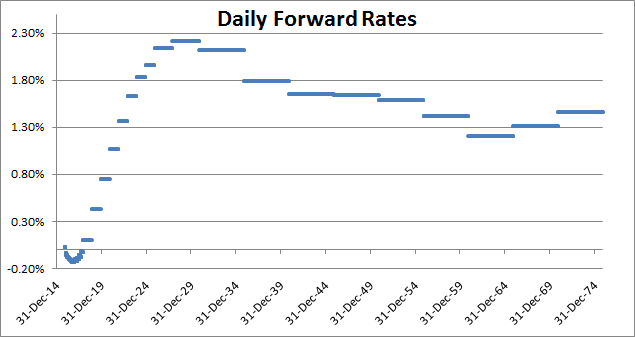
\includegraphics[width=\textwidth]{images/3a.png}
\caption{Piecewise Constant Daily Forward Rates}
\label{fig:3a}
\end{subfigure}
\begin{subfigure}[b]{0.8\textwidth}
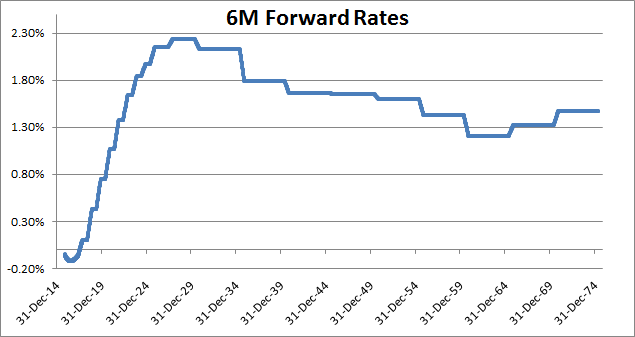
\includegraphics[width=\textwidth]{images/3b.png}
\caption{Stepped 6M Forward Rates}
\label{fig:3b}
\end{subfigure}
\caption{Euribor 6M Curve with Linear interpolation on Log Discount Factors}
\label{fig:3}
\end{figure}

\subsection{Constrained Cubic Spline Interpolation (or "Kruger Scheme")}

Traditional cubic spline interpolation methods describe the unknown function $f$ as a collection of $N-1$ spline functions $f_{i}$ ($i=1,...,N-1$), each one defined on the interval $[t_{i},t_{i+1}]$ through the following criteria:
\begin{itemize}
\item $f_{i}$ is a third order polynomial
\begin{equation}\label{eq:spline}
f_{i}(t)=a_{i}+b_{i}t+c_{i}t^{2}+d_{i}t^{3}
\end{equation}
for $i=1,...,N-1$
\item $f_{i}$ pass through all the known points
\begin{equation}\label{eq:spline1}
f_{i}(t_{i})=y_{i}\text{ , }f_{i}(t_{i+1})=y_{i+1}
\end{equation}
for $i=1,...,N-1$
\item First order derivative is the same for both functions on either side of a point 
\begin{equation}\label{eq:spline2}
f^{\prime}_{i}(t_{i+1})=f^{\prime}_{i+1}(t_{i+1})
\end{equation}
for $i=1,...,N-2$
\item Second order derivative is the same for both functions on either side of a point
\begin{equation}\label{eq:spline3}
f^{\prime\prime}_{i}(t_{i+1})=f^{\prime\prime}_{i+1}(t_{i+1})
\end{equation}
for $i=1,...,N-2$
\end{itemize}
The first equation give us $4N-4$ unknown parameters; the other equations give us $2(N-1)+(N-2)+(N-2)=4N-6$ equations. The two remaining equations are based on a border conditions for the starting and ending points. If we choose the following conditions  
\begin{equation}\label{eq:spline4}
f^{\prime\prime}_{1}(t_{1})=f^{\prime\prime}_{N-1}(t_{N})=0
\end{equation}
the resulting spline is called {\it Natural Spline}.

These interpolation methods suffer of well-documented problems, such as spurious inflection points, excessive convexity, lack of locality and wide oscillations (the spline only alleviates the problem of oscillation seen when fitting a single polynomial). We present now the method of Kruger (\cite{kruger}) which combines the smooth curve characteristics of spline interpolation with non-overshooting behaviour of linear interpolation.

A Constrained Cubic Spline is constructed using equations \ref{eq:spline1}, \ref{eq:spline2}, \ref{eq:spline4} and replacing \ref{eq:spline3} (equal second order derivative at every point) with
\begin{equation}\label{eq:spline5}
f^{\prime}_{i}(t_{i+1})=f^{\prime}_{i+1}(t_{i+1})=f^{\prime}(t_{i+1})
\end{equation}
for $i=1,...,N-2$ where $f^{\prime}(t_{i+1})$ is a specified first order derivative. The result is an interpolated function less smooth but with a specific slope at every point. Intuitively we know the slope of the spline will be between the slopes of the adjacent straight lines. If we define
$$
S_{i}=\frac{y_{i+1}-y_{i}}{t_{i+1}-t_{i}}
$$
a good choice is
\begin{equation}\label{eq:kruger}
f^{\prime}(t_{i})=
\begin{cases}
\frac{2}{\frac{1}{S_{i}}+\frac{1}{S_{i-1}}}&\text{if $S_{i}S_{i-1}\geq 0$} \\
0&\text{if $S_{i}S_{i-1}< 0$}
\end{cases}
\end{equation}
Note that this interpolation scheme preserves monotonicity: in regions of monotonicity of the inputs - three successive increasing or decreasing points - the interpolating function preserves this property. Maximum and minimum points are allowed only on pillars.

The effect of constrained cubic interpolation on zero rates and on the logarithm of discount factors is shown in Figures \ref{fig:4} and \ref{fig:5}. We can notice that the quality of forward rates is really better than the quality achieved with linear interpolation, the best effect obtained interpolating on log discount factors. The heritage of linear interpolation is evident, mainly interpolating on zero rates: the "sawtooth" forwards have become "humps". To reduce this effect the only solution is to increase the number of pillars. Often this is achieved using interpolated quotes.

\begin{figure}
\centering
\begin{subfigure}[b]{0.8\textwidth}
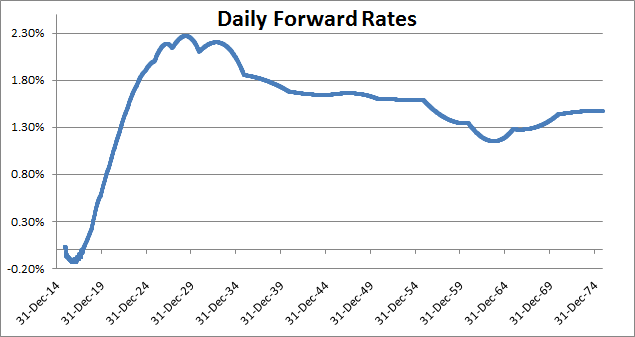
\includegraphics[width=\textwidth]{images/4a.png}
\label{fig:4a}
\end{subfigure}
\begin{subfigure}[b]{0.8\textwidth}
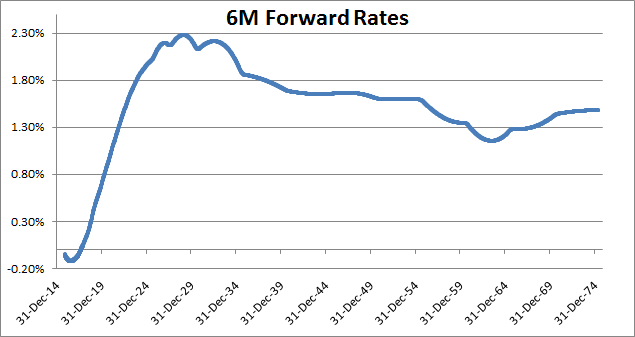
\includegraphics[width=\textwidth]{images/4b.png}
\label{fig:4b}
\end{subfigure}
\caption{Constrained Cubic interpolation on Zero Rates for Euribor 6M Curve}
\label{fig:4}
\end{figure}
\begin{figure}
\centering
\begin{subfigure}[b]{0.8\textwidth}
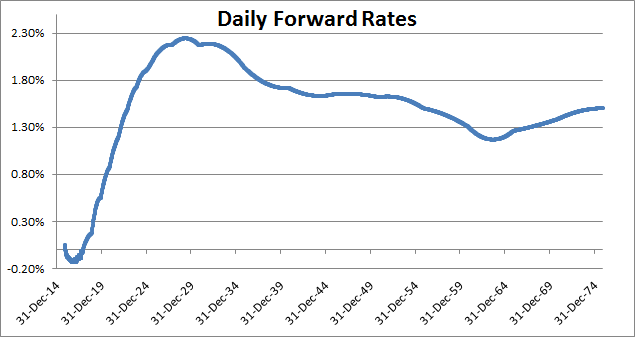
\includegraphics[width=\textwidth]{images/5a.png}
\label{fig:5a}
\end{subfigure}
\begin{subfigure}[b]{0.8\textwidth}
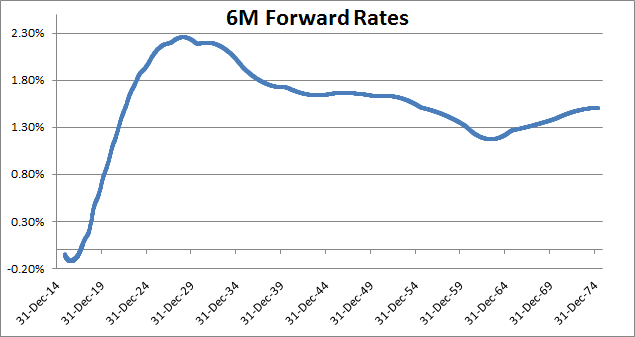
\includegraphics[width=\textwidth]{images/5b.png}
\label{fig:5b}
\end{subfigure}
\caption{Euribor 6M Curve with Constrained Cubic interpolation on Log Discount Factors}
\label{fig:5}
\end{figure}

\subsection{Monotonic Cubic Natural Spline Interpolation (or "Hyman Scheme")}

The method of Hyman or {\it Hyman filter} (\cite{hyman}) attempts to address traditional cubic spline problems in a different way. It's a method that could be applied to any cubic interpolation scheme, for example the cubic natural spline one, to preserve monotonicity. In case of $C^{2}$ interpolation schemes the Hyman filter ensures monotonicity at the expenses of the second derivative of the interpolated function which will no longer be continuous in
the points where the filter has been applied.

Let us briefly sketch how Hyman filter works. When input data are locally monotone (three successive increasing or decreasing points), if the chosen interpolating function is already monotonic, the Hyman filter leaves it unchanged preserving all of its original features; otherwise it changes the slopes locally in order to guarantee monotonicity. When the data are not locally monotone, instead, the interpolated function will have a maximum/minimum at the node. Maximum and minimum points are allowed also between pillars.

The effect of Hyman Filter applied to Cubic Natural Spline Interpolation on zero rates and on the logarithm of discount factors is shown in Figures \ref{fig:6} and \ref{fig:7}. Looking at the smoothness of forward rates, it's clear that this is the best approach from this point of view. 

\begin{figure}
\centering
\begin{subfigure}[b]{0.8\textwidth}
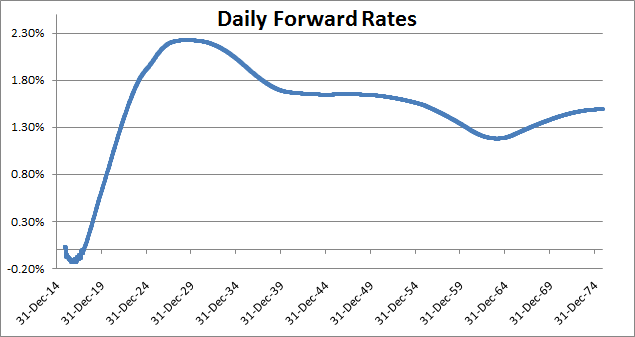
\includegraphics[width=\textwidth]{images/6a.png}
\label{fig:6a}
\end{subfigure}
\begin{subfigure}[b]{0.8\textwidth}
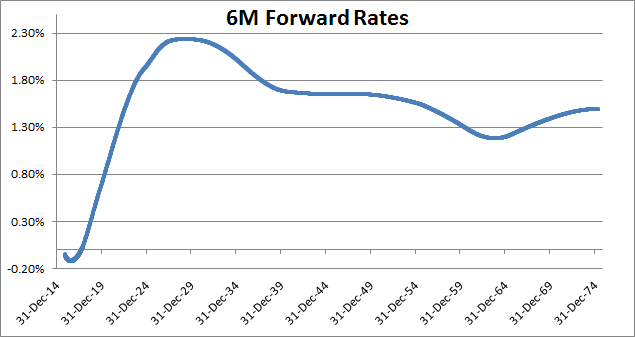
\includegraphics[width=\textwidth]{images/6b.png}
\label{fig:6b}
\end{subfigure}
\caption{Euribor 6M Curve with Monotonic Cubic Natural Spline interpolation on Zero Rates}
\label{fig:6}
\end{figure}
\begin{figure}
\centering
\begin{subfigure}[b]{0.8\textwidth}
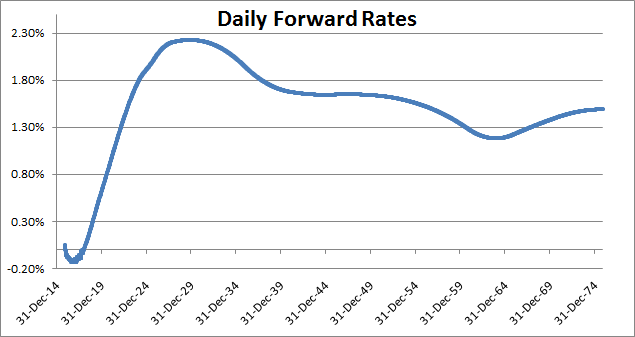
\includegraphics[width=\textwidth]{images/7a.png}
\label{fig:7a}
\end{subfigure}
\begin{subfigure}[b]{0.8\textwidth}
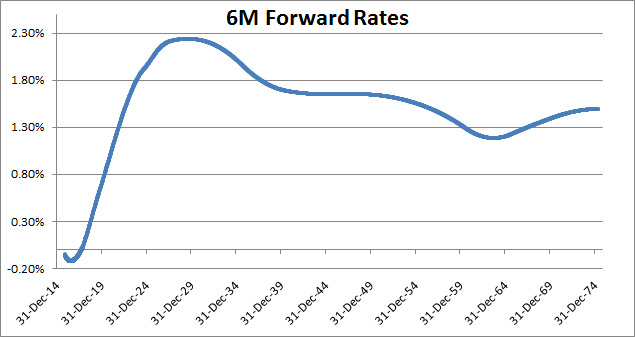
\includegraphics[width=\textwidth]{images/7b.png}
\label{fig:7b}
\end{subfigure}
\caption{Euribor 6M Curve with Monotonic Cubic Natural Spline interpolation on Log Discount Factors}
\label{fig:7}
\end{figure}

\section{Market Instruments Selection}

The selection of calibrating instruments follows two fundamental criteria: 
\begin{enumerate}
\item {\it Homogeneity}: for each currency, build multiple separated sets of Interest Rate Instruments according to the tenor of the underlying rate (1M, 3M, 6M or 12M tenors); instruments depending on two indexes are allowed (for instance Basis Swaps).  
\item {\it Maximum Liquidity}: for each currency-tenor pair, the chosen instruments may overlap in some sections; in order to define a subset of (mostly) non-overlapping instruments preference must be given to the more liquid ones.
\end{enumerate}

You can refer to \cite{ametranobianchetti} or \cite{mazzocchi} for a review of most important calibrating instruments and corresponding bootstrapping equations.

\section{Synthetic Instruments}

A synthetic bootstrapping instrument is an instrument that is not directly quoted on the market but can be built starting from other quoted instruments. We can at least define two classes of synthetic instruments.

\subsection{Synthetic Interpolated Instruments}\label{sec:synthinterp}
These are instruments whose quotes can be determined directly interpolating on available market quotes. For example, if we need an IRS with maturity 27 years and it is not quoted by the market, we can choose an interpolation method and interpolate 25 years swap and 30 years swap quotes to find the missing quote. This approach is quite rough and can generate very bad forward rates.

We can define another kind of synthetic interpolated instruments. Imagine you have already calibrated a discounting curve and a forwarding curve of a certain tenor. Now you are able to price all the instruments related to that specific tenor, included non quoted ones. For example, you have calibrated your forwarding curve using Basis Swaps because Swaps are not quoted by the market. With this curve plus an appropriate discounting curve you can calculate synthetic Swap quotes and use them to perform a second bootstrap. Clearly the product of this second calibration will be different from the product of the first one. Another example. You have to calibrate using few Swap quotes because the market doesn't quote a lot of maturities. After that you can calculate synthetic Swaps quotes for every maturity you want and use the whole set of Swap quotes to perform a second different calibration. In this case we do not interpolate directly market quotes but we interpolate the bootstrapped curve. We will see i chapter \ref{chap:4} why it is important to define this kind of instruments.

\subsection{Synthetic Deposits}\label{sec:synth}
As anticipated in section \ref{sec:description}, it may happen that we have to describe each forward curve $C_{x}$ of our framework with pseudo-discount factors. When $x=ON$ this kind of description is consistent with the role of $C_{ON}$ as discount curve of the framework. Hence we can consider to have at our disposal the discounting curve $C_{ON}$. Conversely when $x\neq ON$ we have to manage the arbitrariness of the function $P_{x}(t;s)$ imposing more conditions (as explained in section \ref{sec:description}). We first show with a practical example what happens if we do not add more constraints. 

Let $C_{6M}$ be the Euribor $6M$ forwarding curve. We can try to calibrate this curve using only the available market quotes (6M FRA and Swaps) and a specific interpolation algorithm. As shown in Figure \ref{fig:15} this approach leads to bad results even using sophisticated interpolation methods (Hyman scheme on Log Discount Factors): daily forward rates have an oscillatory behavior in the first section of the curve; consequently $6M$ forward rates curve shows humps in the same section. The reason of this behavior could be that each market FRA quote determines two discount factors. For example, the $1X7$ FRA quote fixes the values for $P_{6M}(t;t+1M)$ and $P_{6M}(t;t+7M)$: this is possible (using the iterative procedure mentioned in section \ref{sec:algo}) but we do not have control on the final result, which is completely determined by the interpolation method. For more details you can refer to \cite{mazzocchi}.

\begin{figure}
\centering

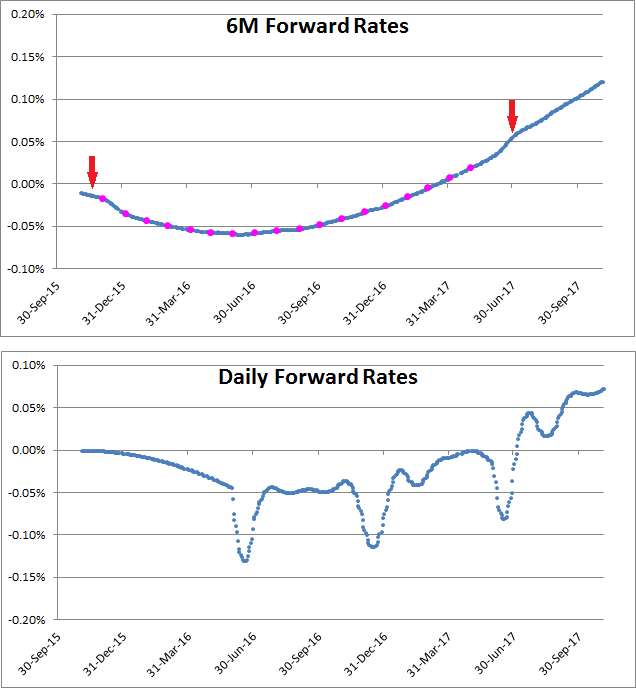
\includegraphics[width=\textwidth]{images/15.png}

\caption{Euribor $6M$ Curve calibrated using only the available market quotes and interpolating with the Hyman scheme on Log Discount Factors (Evaluation Date: 30 October 2015). Daily forward rates curve in the first section has an oscillatory behavior; $6M$ forward rates curve shows humps in the same section (red arrows). The pink dots represent the FRA market quotes used for calibration.}
\label{fig:15}
\end{figure}

We can try to improve the method using the underlying index fixing value as best proxy of the discrete forward $F_{x}(t;t,t+x)$. In our example, taking into account this information, we can fix the pseudo-discount factor $P_{6M}(t;t+1M)$ interpolating between the two nodes $P_{6M}(t;t)=1$ and 
$$
P_{6M}(t;t+6M)=\frac{1}{1+\tau_{x}(t,t+6M)F_{6M}(t;t+6M)}
$$
Then, using this value and the $1X7$ FRA quote, we can determine $P_{6M}(t;t+7M)$. First of all, notice that this method can be used only if we are interpolating on discount factors (zero rates and instantaneous forward rates are not defined in $s=t$). Secondly, as explained in \cite{ametranomazzocchi} and \cite{mazzocchi}, also this method produces bad results for at least two reasons: the fixing value used to calculate the discount factor $P_{x}(t;t+x)$ does not change during the day and so is not really representative of the simple forward $F_{x}(t;t,t+x)$ implicitly quoted by the market; most of the work is still done by the interpolation method.

For all these reasons we usually try to solve the "arbitrariness issue" before starting calibration. We choose to fix the shape of $C_{x}$ on the first $x$ interval $[t,t+x)$ ($t=spot(today)$ is the curve reference date) and we have to do this with a reliable method ensuring the smoothness of the curve and consistency with the available $x$-tenor market quotes. Notice that a quoted instrument with underlying rate of tenor $x$ has maturity date not earlier than $t+x$. For example, if $x=6M$ the first available instrument is the $1X7$ FRA (as said before) whose maturity date falls outside the chosen interval $[t,t+x)$. So we can't use directly market quotes to determine the short term part of $C_{x}$.

The basic idea is to build the short term part of the curve with a shift of $C_{ON}$ consistent with the available $x$-tenor market quotes. Since we can't use directly market quotes (as explained before) we define a set of $n$ deposits with maturity dates that fall inside $[t,t+x)$ an use them to bootstrap the first section of the curve using the equation
\begin{equation}\label{eq:synth1}
P_{x}(t;s_{i})=\frac{1}{1+r^{i}_{x}\tau_{x}(t,s_{i})}
\end{equation}
where $r^{i}_{x}$ and $s_{i}\in [t,t+x)$ are the quote and the maturity date of the $i$-th instrument respectively. In practice we have to calculate the quotes $\{r^{i}_{x}\}_{i=1,...,n}$ using the available market quotes. Notice that
\begin{equation}\label{eq:synth2}
r^{i}_{x}=\frac{1}{\tau_{x}}\left(\frac{1}{P_{x}(t;s_{i})}-1\right)\stackrel{\ref{eq:fwd}}{=} F_{x}(t;t,s_{i})
\end{equation}
so that we can determine the whole set of synthetic quotes fixing the shape of simple forward rates on $[t,t+x)$. In order to do this we define the {\it continuous compounded basis} $\delta_{x}$ and the {\it integrated continuous compounded basis} $\Delta_{x}$ as
\begin{align}
\delta_{x}(t;u)&=f_{x}(t;u)-f_{ON}(t;u) \label{eq:synth3}\\
\Delta_{x}(t;s_{1},s_{2})&=\int_{s_{1}}^{s_{2}}\delta_{x}(t;u)du \label{eq:synth3bis}
\end{align}
where $u,s_{1},s_{2}\geq t$, and then calculate
\begin{equation}\label{eq:synth4}
\begin{split}
F_{x}(t;s_{1},s_{2})&=\frac{1}{\tau_{x}(s_{1},s_{2})}\left(e^{\int_{s_{1}}^{s_{2}}f_{ON}(t;u)du}e^{\int_{s_{1}}^{s_{2}}\delta_{x}(t;u)du}-1\right)=\\
&=\frac{1}{\tau_{x}(s_{1},s_{2})}\left(\left(1+F_{ON}(t;s_{1},s_{2})\tau_{x}(s_{1},s_{2})\right)e^{\int_{s_{1}}^{s_{2}}\delta_{x}(t;u)du}-1\right)=\\
&=\frac{1}{\tau_{x}(s_{1},s_{2})}\left(\left(1+F_{ON}(t;s_{1},s_{2})\tau_{x}(s_{1},s_{2})\right)e^{\Delta_{x}(t;s_{1},s_{2})}-1\right)
\end{split}
\end{equation}
Equivalently
\begin{equation}\label{eq:synth5}
\Delta_{x}(t;s_{1},s_{2})=\ln \left(\frac{1+F_{x}(t;s_{1},s_{2})\tau_{x}(s_{1},s_{2})}{1+F_{ON}(t;s_{1},s_{2})\tau_{x}(s_{1},s_{2})}\right)
\end{equation}

Now it's simple to understand how we can proceed to determine the synthetic quotes $\{r^{i}_{x}\}_{i=1,...,n}$:
\begin{enumerate}
\item First we assume a functional form for $\Delta_{x}$ (or equivalently $\delta_{x}$) with N parameters; usually the continuous compounded $ON$-$x$ basis is  approximated with a polynomial of degree $N-1$ with $N$ parameters
$$
\delta_{x}(t;u)=\sum_{j=1}^{N}\alpha_{j}\tau_{x}(t;u)^{j-1}
$$
so that
$$
\Delta_{x}(t;s_{1},s_{2})=\sum_{j=1}^{N}\left[\frac{\alpha_{j}}{j}\left(\tau_{x}(t;s_{2})^{j}-\tau_{x}(t;s_{1})^{j}\right)\right]
$$
\item Secondly we calculate $N$ values $\{\Delta_{x}(t;t_{j},t_{j}+x)\}_{j=1,...,N}$ via equation \ref{eq:synth5} starting from
\begin{itemize}
\item $N$ available market quotes $F_{x}(t;t_{j},t_{j}+x)$;
\item $N$ corresponding forward rates $F_{ON}(t;t_{j},t_{j}+x)$ calculated using $C_{ON}$.
\end{itemize}
\item We then calibrate $\Delta_{x}$ parameters using the $N$ values $\{\Delta_{x}(t;t_{j},t_{j}+x)\}_{j=1,...,N}$.
\item Finally we calculate our synthetic deposits quotes $\{r^{i}_{x}\equiv F_{x}(t;t,s_{i})\}_{i=1,...,n}$ using equation \ref{eq:synth4} and
\begin{itemize}
\item $n$ corresponding forward rates $F_{ON}(t;t,s_{i})$ calculated using $C_{ON}$;
\item $n$ corresponding basis values $\Delta_{x}(t;t,s_{i})$ calculated using the calibrated basis $\Delta_{x}$.
\end{itemize}
These quotes are used as an input of the bootstrapping procedure as they were real market quotes. 
\end{enumerate}
The result of this approach applied to the Euribor $6M$ curve is shown in Figure \ref{fig:16}. The difference with Figure \ref{fig:15} is evident.

\begin{figure}
\centering

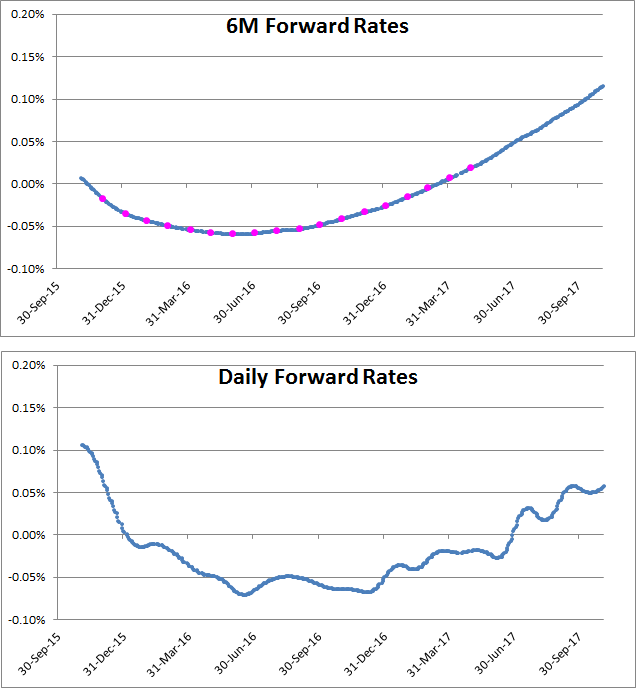
\includegraphics[width=\textwidth]{images/16.png}

\caption{Euribor $6M$ Curve calibrated using synthetic deposits quotes, the available market quotes and interpolating with the Hyman scheme on Log Discount Factors (Evaluation Date: 30 October 2015). Daily forward rates curve in the first section has less oscillations; $6M$ forward rates curve do not show humps. The pink dots represent the FRA market quotes used for calibration.}
\label{fig:16}
\end{figure}

The quotes used for $\Delta_{x}$ calibration must be selected carefully. For example, the underlying index fixing value must not be taken into account directly because (as said before) is not representative of the discrete forward $F_{x}(t;t,t+x)$ quoted by the market. Also, to improve synthetic deposits calculation, it's possible to model "jumps" ({\it Turn Of Year} and {\it End of Month} effects). For more details you can refer to \cite{ametranomazzocchi} and \cite{mazzocchi}.

\section{First order sensitivities (or Deltas)}\label{sec:deltas}

Curves are not only accounting tools but also risk management tools to analyse the risks. We concentrate on first order risks called {\it deltas}. Let's consider a portfolio of interest rate derivatives depending on our set of calibrated curves $\{C_{i}\}_{i=1,...,n}$ each characterised by a time grid $\{T_{ij}\}_{j=1,...,k_{i}}$ and a set of bootstrapping instruments with market quotes $\{Q_{ij}\}_{j=1,...,k_{i}}$. Defining $Q=\{Q_{ij}\}_{i,j}$ as the entire set of bootstrapping market quotes, the price of our portfolio at time $t$ will be denoted by $\Pi(t;Q)$.

The portfolio's delta is the first order estimate of the price change for a change of the quotes of the instruments in the bootstrapping basket. We now have to make an assumption on possible changes of quotes.

Usually by quote we mean a rate or a price: an interest rate swap quote is always a rate; futures, instead, are quoted in terms of price. The simplest change we can imagine is a rate shift $\delta$, which for example correspond to a future price shift of $-100\cdot\delta$. Usually $\delta=1 bps$, which at present is the choice of our front office system.

We assume that all the possible quote changes are the ones just described; we will indicate with $\delta_{ij}$ the shift corresponding to the quote $Q_{ij}$ (if $\delta_{ij}=\delta$ in case of a rate, $\delta_{ij}=-100\cdot\delta$ in case of price and so on).
   
When one single quote $Q_{ij}$ is shifted, the first order estimation of the price change is
\begin{equation}\label{eq:bucketdelta}
\Delta_{ij}^{\Pi}(t;Q)=\frac{\partial \Pi}{\partial Q_{ij}}\delta_{ij}
\end{equation}
that is called {\it bucketed delta for pillar $T_{ij}$}. We can define also the {\it partial delta for curve $C_{i}$} as
\begin{equation}\label{eq:partialdelta}
\Delta_{i}^{\Pi}(t;Q)=\sum_{j=1}^{k_{i}}\Delta^{\Pi}_{ij}(t;Q)
\end{equation}
which corresponds to a parallel movement of the set of quotes associated to the curve $C_{i}$ (every quote related to curve $C_{i}$ is shifted as explained before). Finally the {\it total delta} is defined by
\begin{equation}\label{eq:totaldelta}
\Delta^{\Pi}(t;Q)=\sum_{i=1}^{n}\Delta^{\Pi}_{i}(t;Q)
\end{equation}
which corresponds to a parallel movement of the whole set of quotes $Q$. Usually the derivatives $\frac{\partial \Pi}{\partial Q_{ij}}$ are calculated using a finite differences method. The shift $h$ used to perform the calculation must be selected carefully: a shift too big or too small could negatively affect calculation.

Within a curve-based pricing framework, the value of $\Pi$ doesn't depend directly on market rates $Q$ but indirectly through discount factors and forward rates appearing in the corresponding pricing formulas. Since forward rates could be written in terms of their associated discount factors and since discount factors could be written in terms of their corresponding zero rates, we may think that $\Pi$ depends directly on a set of zero rates $\{z_{ij}\}$. Note that a single zero rate $z_{ij}$ may depend on more than one single market quote due to non-local effects in bootstrapping. For the sake of simplicity, let us neglects effects due to exogenous discounting so that each zero rate depends only on market quotes related to its specific curve. In this case we can write
\begin{equation}
\frac{\partial \Pi}{\partial Q_{ij}}=\sum_{h=1}^{k_i}\frac{\partial z_{ih}}{\partial Q_{ij}}\frac{\partial \Pi}{\partial z_{ih}}
\end{equation}
So in matrix notation we have
\begin{equation}
\Delta_{i}^{\Pi}(t;Q)=\delta_{i}\cdot J_{i}\cdot \nabla_{i}\Pi
\end{equation}
where
\begin{equation}
J_{i}=\left[\frac{\partial z_{ih}}{\partial Q_{ij}}\right]_{jh}
\end{equation}
is the {\it Jacobian Matrix} for curve $C_{i}$,
\begin{equation}
\nabla_{i}=\left[\frac{\partial}{\partial z_{ih}}\right]_{h}
\end{equation}
is the {\it gradient operator} for curve $C_{i}$ and
\begin{equation}
\delta_{i}=\left[\delta{ij}\right]_{j}
\end{equation}
Finally
$$
\Delta^{\Pi}(t;Q)=\sum_{i=1}^{n}\delta_{i}\cdot J_{i}\cdot \nabla_{i}\Pi
$$
This is the formula used by our front office systems to perform the calculation. Obviously formulas which consider exogenous discounting are more sophisticated but it is not our main purpose presenting them here. 

Once the partial and total deltas has been computed, we want to hedge our portfolio by trading appropriate amounts of hedging instruments (each one with unit nominal amount). Typically the set of hedging instruments for curve $C_{i}$ is a subset of the most liquid bootstrapping instruments of $C_{i}$ but their selection is subjective and is part of an interest rate trader work. Note that for each instruments used in the curve construction only a delta with respect to the instrument itself will appear because its quote is not affected by other instruments in the basket. Hedging amounts are chosen in such a way that the total portfolio (consisting of the original portfolio plus the appropriate amount of each hedging instrument) satisfies the zero delta condition. 

Different interpolation methods may lead to huge differences in bucketed deltas. If a method implies that you have to use ten year swap to hedge a seven month swap, probably is not the right method. We will now analyze the impact of interpolation choice on deltas calculation calibrating a discount curve $C_{ON}$ using the same data but different interpolation techniques. In particular we compare
\begin{itemize}
\item Linear interpolation on zero rates
\item Linear interpolation on logarithm of discount factors
\item Constrained Cubic interpolation on zero rates
\item Constrained Cubic interpolation on logarithm of discount factors
\item Monotonic Cubic Natural Spline Interpolation on zero rates
\item Monotonic Cubic Natural Spline on logarithm of discount factors
\end{itemize}
Then, for each interpolation method we calculate deltas for a 5Y OIS with 2M forward start (notional 100000000) and look at the differences. Results are shown in figure \ref{fig:8}.

\begin{figure}
\centering
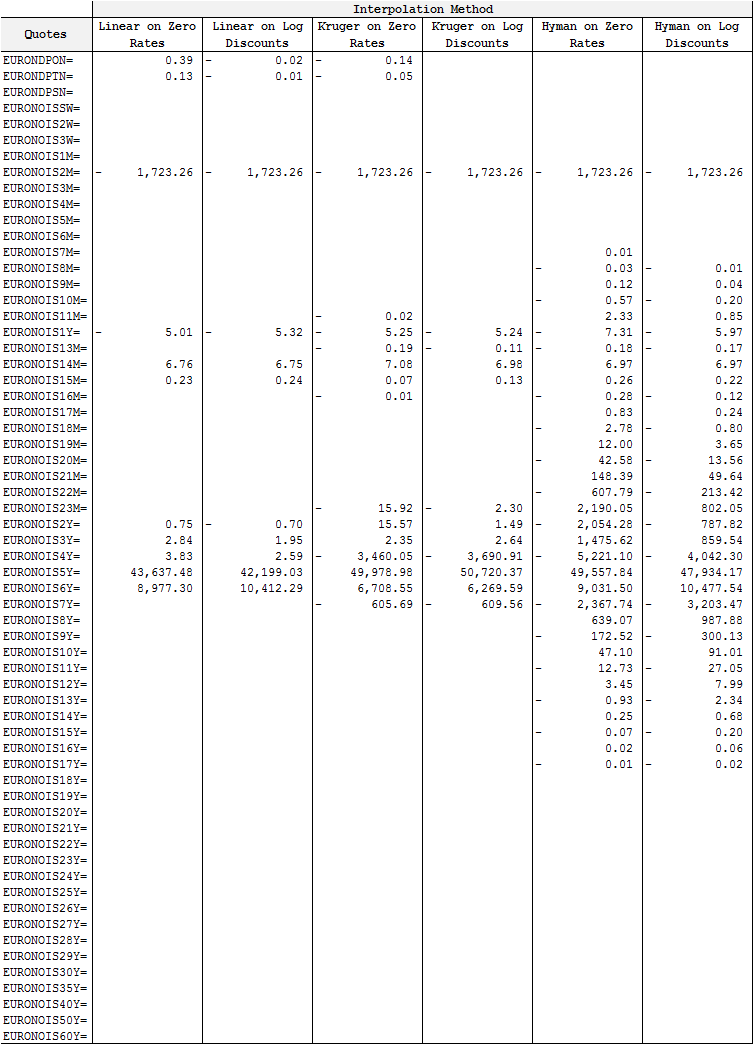
\includegraphics[width=\textwidth]{images/8.png}
\caption{Deltas for a 2M Forward Start 5Y OIS with different interpolation methods (Evaluation Date 30 October 2015)}
\label{fig:8}
\end{figure}

It's clear from our example that local methods are the best choice from an hedging point of view because they imply an intuitive and simple hedging strategy (deltas are concentrated around pillars which correspond to the start and end dates of the instrument). Unfortunately we know from section \ref{sec:interpolation} that these methods don't produce good forward rates. In the same section we claimed that Hyman scheme produces the best forward rates but this new test shows that its non-locality level is too high for hedging purposes. The best compromise seems to be the Kruger scheme; we will apply it to zero rates and not on to the logarithm of discount factors because this last method has shown in some market conditions a lot of instability concerning deltas calculation (September-December 2014). The residual problem is the humped behavior of forward rates but we will address it in next chapter.




